\section{Laufzeitanalysen}

Das System, auf dem der Algorithmus getestet wurde, ist wie folgt ausgestattet:
\begin{itemize}
	\item 2x Intel Xeon CPU E5-2667 0 @ 2.90GHz
	\item 8x 16 GB DDR3 @ 1600MHz
	\item 2x Nvidia Tesla K20c
	\item Dell 0F5XM3 Server Motherboard
\end{itemize}


\begin{figure}
	\centering
	\vspace{-1cm}
	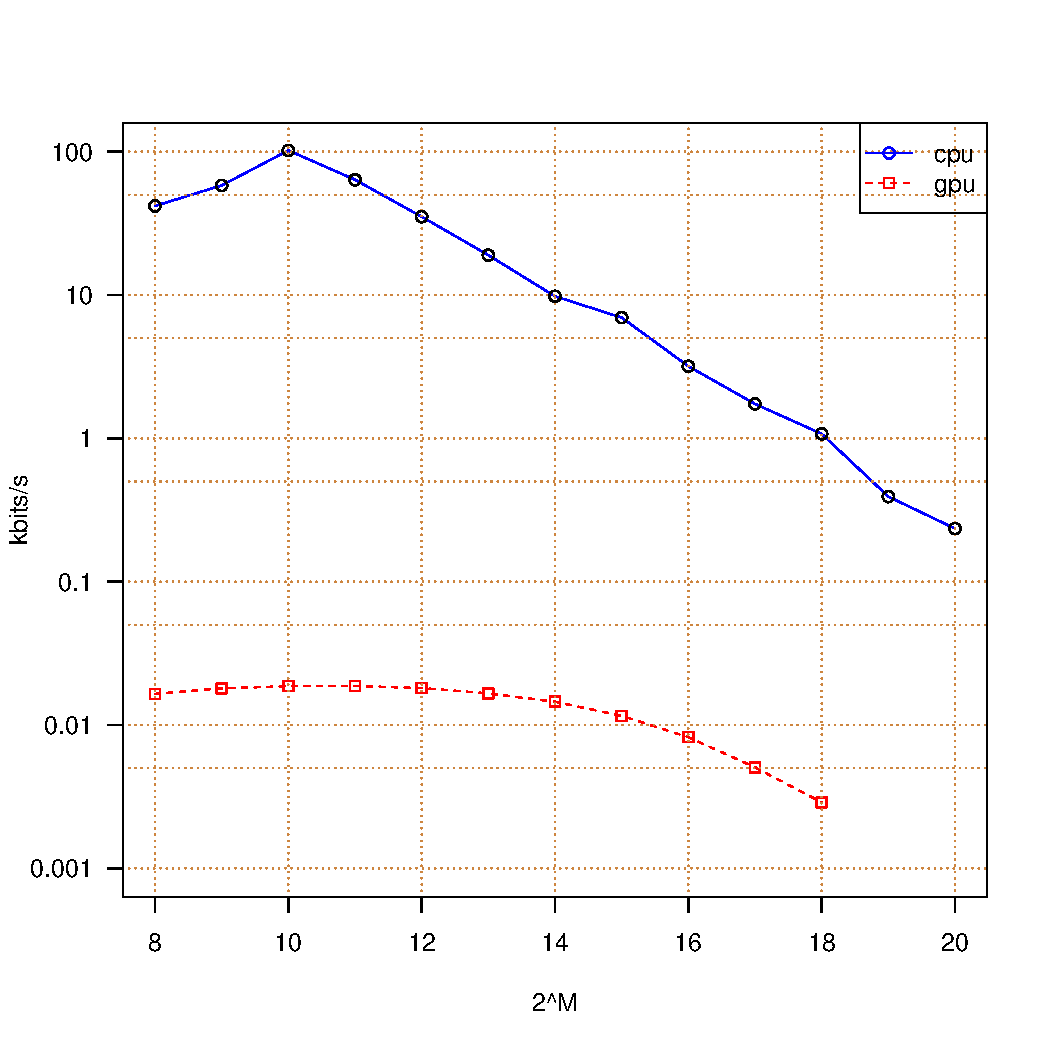
\includegraphics[scale=.5]{combined.pdf}
	\caption{Laufzeit CPU vs GPU}
	\label{fig:laufzeitCpuGpu}
\end{figure}

Um die Performance des Extraktors zu messen und zu vergleichen wurde ein Shellscript geschrieben. Als Testparameter wurde $m$, die Anzahl der zu extrahierenden Bits, gew"ahlt, wobei $m = 2^M$ und $M \in \{8, \dots, 20\}$. Die gew"ahlte Seedl"ange $n$ ist immer um den Faktor $16$ gr"o"ser als $m$. Um den Einfluss einzelner Ausrei"ser zu mindern, wird der Test mehrfach wiederholt und das daraus resultierende Arithmetische Mittel betrachtet. Abbilddung \ref{fig:laufzeitCpuGpu} ist ein Plot der Ergebnisse des Tests. Die x-Achse des Liniendiagramms gibt die Anzahl der zu extrahierenden Bits an und die y-Achse zeigt die gemessene Performance in \emph{kbits/s} auf eine logarithmischen Skala.

\begin{figure}[h]
	\vspace{-.5cm}
	\begin{minipage}[b]{0.5\textwidth} 
		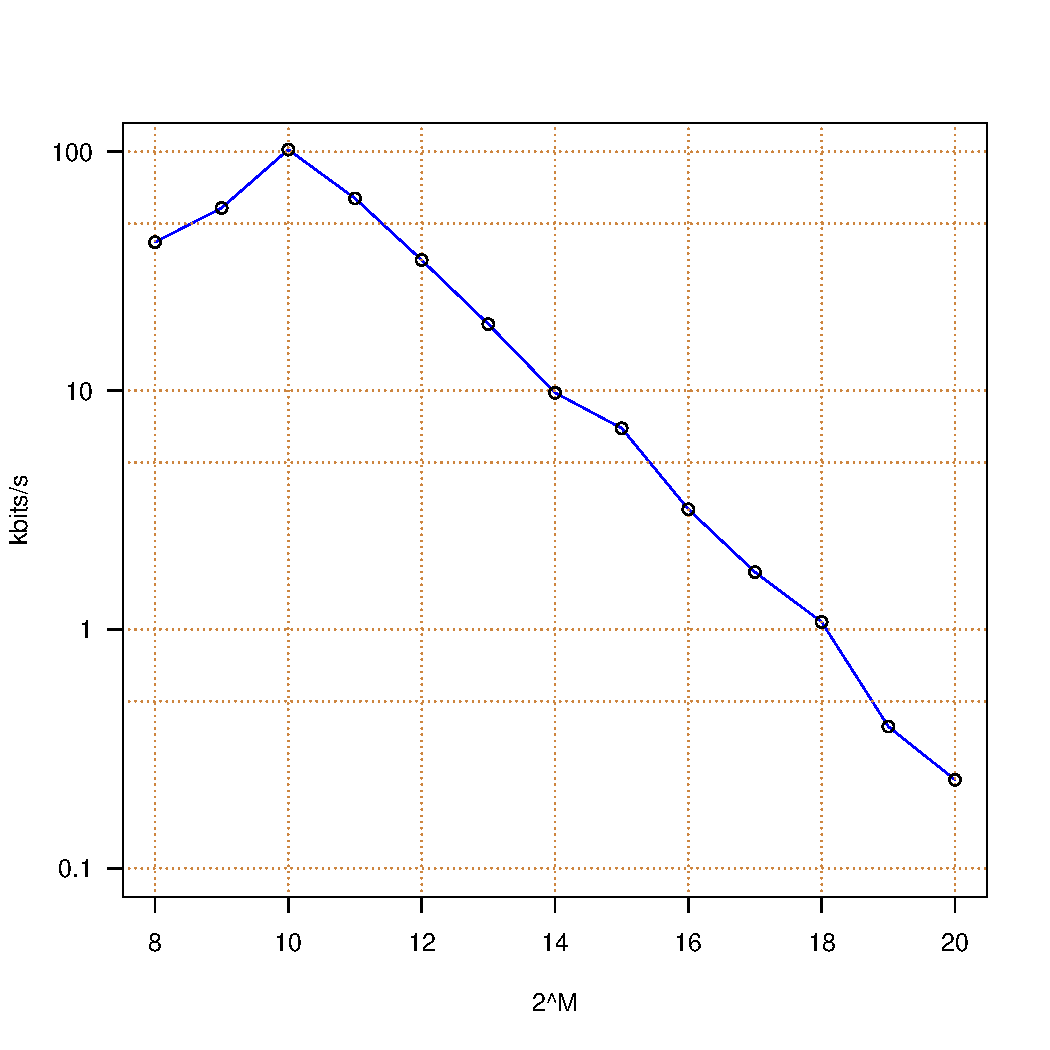
\includegraphics[width=\textwidth]{rsh.pdf}
		\caption{Laufzeit CPU}
		\label{fig:laufzeitCpu} 
	\end{minipage}
	% Auffüllen des Zwischenraums
	\hfill
	\begin{minipage}[b]{0.5\textwidth}
	% \textwidth bezieht sich nun auf die Minipage
		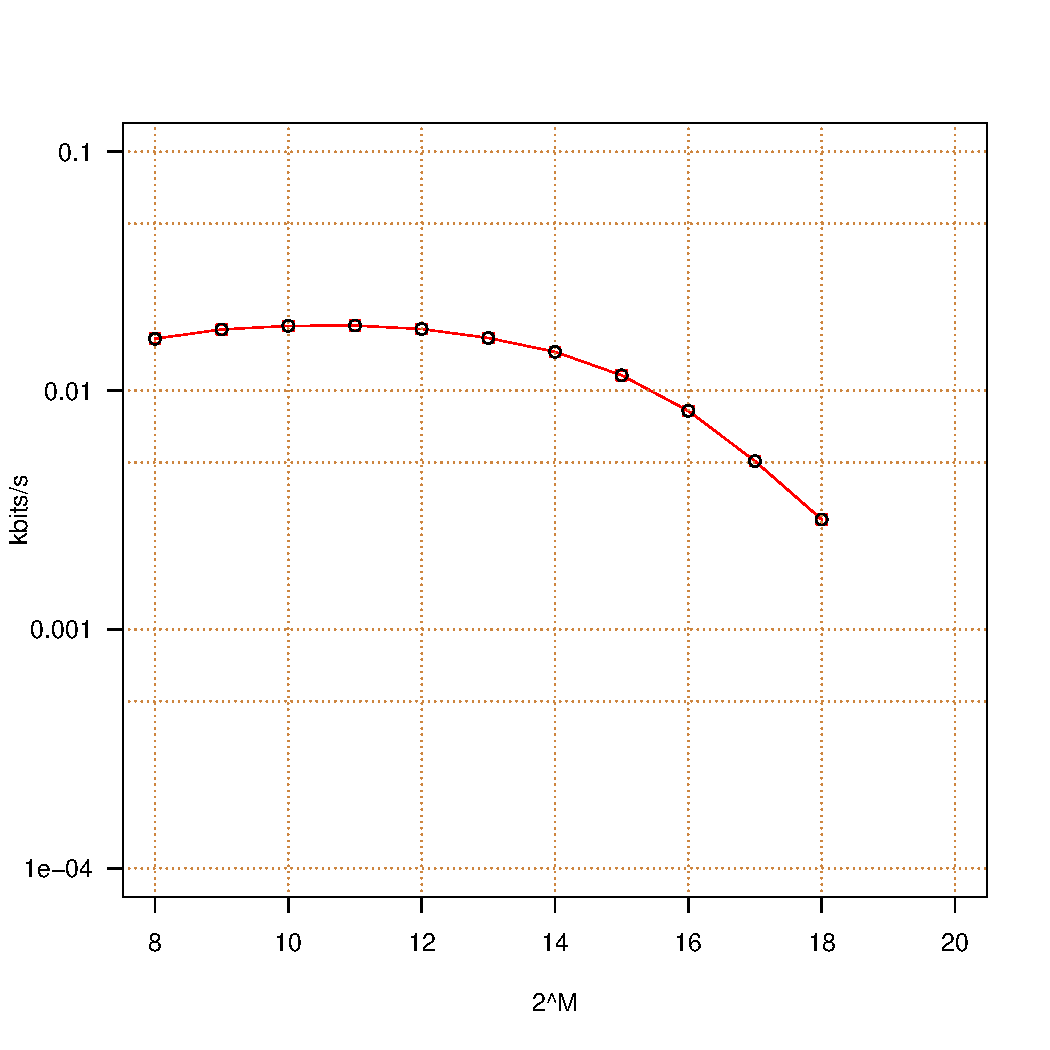
\includegraphics[width=\textwidth]{rsh_cuda.pdf}
		\caption{Laufzeit GPU}
		\label{fig:laufzeitGpu} 
	\end{minipage}
\end{figure}

Abbildung \ref{fig:laufzeitCpu} und \ref{fig:laufzeitGpu} zeigen die beiden Kurven zur besseren Vergleichbarkeit nebeneinander mit dem gleichen Raster. Die beiden Testparametern $M=19$ und $M=20$ f"uhren in der aktuellen Implementierung zu \emph{Segmentaion Faults}. Dies fiel beim Entwickeln nicht auf, da aus Zeitgr"unden nur kleine Werte f"ur $m$ und $n$ getestet wurden (die Extraktion von $2^{18}$ bits dauert ca. 30 Stunden).

Aus den gemessenen Werten geht hervor, dass der CPU Algorithmus um den Faktor $10^3$ schneller ist. Die Kurve des GPU-Algorithmus bleibt allerdings "uber einen gr"o"seren Wertebereich von $M$ stabil und beginnt erst bei $M=15$ so stark zu sinken wie der CPU-Algorithmus ab $M=10$. Da der GPU-Algorithmus noch einiges Potential zur Optimierung bietet, besteht durchaus die Chance vergleichbare Extraktionsraten zu erreichen.
